\chapter{SYSTEM DESIGN }

\section{Use case model}
\begin{figure}[H]
    \centering
    % 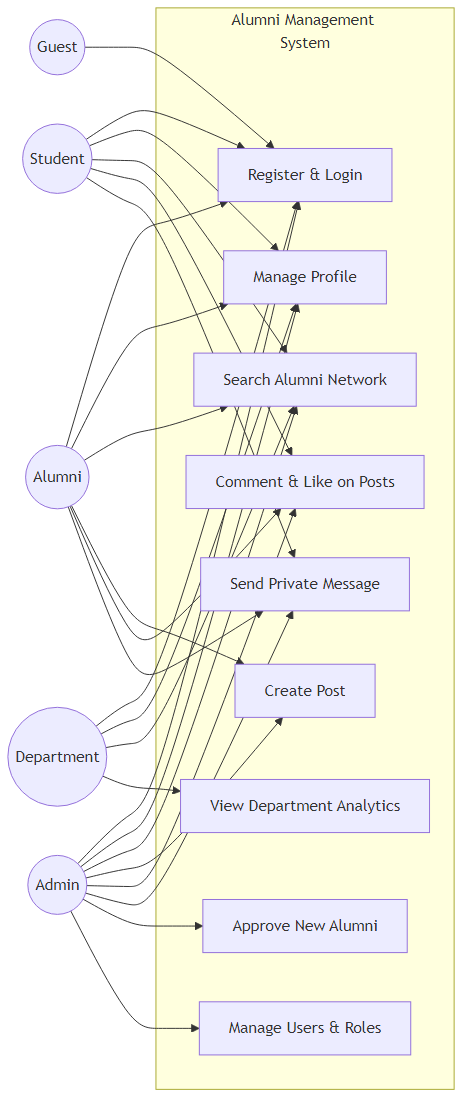
\includegraphics[width=1\textwidth,height=0.6\textwidth]{use_case.png} % Place your actual image here
    \framebox[1\textwidth]{\rule{0pt}{0.4\textwidth} \Huge Placeholder for Use Case Diagram}
    \caption{Use case Diagram}
    \label{fig:Use_case}
\end{figure}
The use case model defines the core interactions between actors and the system, detailing workflows such as user registration and direct messaging.

\section{Project Design}
System design is the process of defining the architecture, components, interfaces, and other characteristics of a system or component. For the Alumni System, the design focuses on creating an intuitive networking environment reminiscent of professional platforms like LinkedIn.\\\\
In the Alumni System, the design focuses on ensuring that user interactions—such as making a post or sending a message—are fast and responsive. The interface dynamically adapts depending on whether the user is an Admin, a Student, or a Department to ensure optimal usability.

\subsection{UI Design}
The User Interface is designed with a "vibrant, modern, and professional" aesthetic.
\begin{itemize}
    \item \textbf{Dashboard:} Features a clean, single-column feed of interactive Post Cards, allowing users to scroll through updates smoothly.
    \item \textbf{Navigation:} A sticky top navigation bar houses rapid-access tools: a global search bar, profile picture dropdown, and a dynamic Notification Bell that reveals recent activity.
    \item \textbf{Profiles:} Rendered as stacked cards, clearly separating "About", "Academic Background", "Skills", and the user's historical "Activity/Posts".
\end{itemize}

\subsection{Post \& Feed Design}
The design of the content feed prioritizes visual engagement. The system uses a centralized reusable Blade component (\texttt{post-card.blade.php}) ensuring that whether a post is viewed on the main Dashboard or on a specific User's Profile, it looks completely identical and professional. Posts support rich media (images and videos) and feature interactive elements for Liking and Commenting, styled with SVG icons and subtle hover animations for a premium feel.

\subsection{Notification System Design}
The Notification engine shifts away from basic manual database queries to an integrated, universal alert system. 
\begin{itemize}
    \item \textbf{Implementation:} Utilizing Laravel's built-in \texttt{Notification} facade and the \texttt{database} channel.
    \item \textbf{Triggers:} Custom Notification classes (\texttt{NewMessageNotification}, \texttt{NewPostNotification}) are fired directly from the Controllers when a successful action occurs.
    \item \textbf{User Experience:} These raw database alerts are beautifully rendered via a custom dropdown menu in the navigation bar, formatting timestamps dynamically (e.g., "5 minutes ago") and visually bolding unread items. A one-click "Mark as Read" instantly clears the user's queue.
\end{itemize}
